\chapter{Geodesics in Schwarzschild spacetime}
\label{s:ges}
\index{geodesic!in Schwarzschild spacetime}

\minitoc

\section{Introduction}

We have already investigated some geodesics in Schwarzschild spacetime in
Chap.~\ref{s:sch}, namely
the radial null geodesics (Sec.~\ref{s:sch:rad_null_geod}).
Here, we perform a more extensive study. In particular we investigate timelike
geodesics, which are of primordial physical importance, since they represent
orbits of planets or stars around the black hole or worldlines of
intrepid observers freely falling into the black hole.

\section{Geodesic motion}

Let $\Li$ be a geodesic\footnote{The definition and basic properties of geodesics
are recalled in Appendix~\ref{s:geo}.} of Schwarzschild spacetime
$(\M,\w{g})$. We shall assume that $\Li$ is causal, i.e. either timelike or null\footnote{As
shown in Sec.~\ref{s:geo:def}, a geodesic cannot be partly timelike and partly
null.}. It therefore can be considered as the worldline
of some particle $\mathscr{P}$, either massive
($\Li$ timelike) or masseless ($\Li$ null).


\subsection{First integrals of motion}

The Schwarzschild spacetime $(\M,\w{g})$ is static and spherically symmetric; the
Killing vector $\w{\xi}$ associated with the staticity (cf. Sec.~\ref{s:sch:static_spher})
and the Killing vector $\w{\eta}$ associated with the rotation symmetry along any
axis, give birth to two conserved quantities along $\Li$:
\begin{greybox}
The scalar products
\begin{subequations}
\label{e:ges:conserved_quantities}
\begin{align}
& \encadre{\veps := - \w{\xi}\cdot \w{p} = - \w{g}(\w{\xi},\w{p}) } \label{e:ges:conserved_energy} \\
& \encadre{\ell := \w{\eta}\cdot \w{p} = \w{g}(\w{\eta},\w{p}) } , \label{e:ges:conserved_angu_mom}
\end{align}
\end{subequations}
where $\w{p}$ is the 4-momentum of particle
$\mathscr{P}$ (cf. Sec.~\ref{s:fra:worldlines}),
are constant along the geodesic $\Li$.
The scalar $\veps$ is called $\mathscr{P}$'s
\defin{conserved energy}\index{conserved!energy}\index{energy!conserved --}
or \defin{energy at infinity}\index{energy!at infinity},
while $\ell$ is called $\mathscr{P}$'s \defin{conserved angular momentum}\index{conserved!angular momuntum}\index{angular momentum!conserved --}
or \defin{angular momentum at infinity}\index{angular momentum!at infinity}.
\end{greybox}
\begin{proof}
The 4-momentum $\w{p}$ is a tangent vector associated with an affine parameter
of $\Li$, i.e. it obeys the geodesic equation (\ref{e:fra:p_geodesic}).
The constancy of $\veps$ and $\ell$ follow then from the generic property (\ref{e:geo:g_xi_v_const})
of geodesics in presence of a spacetime symmetry.
\end{proof}
In coordinates $(t,r,\th,\ph)$ adapted to the spacetime symmetries,
i.e. coordinates such that $\w{\xi} = \wpar_t$ and $\w{\eta}=\wpar_\ph$, like the Schwarzschild-Droste
coordinates or the Eddington-Finkelstein ones, one can rewrite
(\ref{e:ges:conserved_quantities})
in terms of the components $p_t = g_{t\mu} \, p^\mu$ and $p_\ph = g_{\ph\mu} \, p^\mu$
of the 1-form $\uu{p}$ associated to $\w{p}$ by metric duality:
\begin{subequations}
\begin{align}
& \veps = - p_t \\
& \ell = p_\ph
\end{align}
\end{subequations}
Indeed, in such a coordinate system, $\xi^\mu =  \delta^\mu_{\ \, t}$
and $\eta^\mu = \delta^\mu_{\ \, \ph}$, so that $\veps = -g_{\mu\nu} \, \xi^\mu p^\nu = -g_{t\nu} \, p^\nu = -p_t$
and $\ell = g_{\mu\nu} \, \eta^\mu p^\nu = g_{\ph\nu} \, p^\nu = p_\ph$.


It is worth stressing that $\veps$ is not a genuine energy, i.e. it is not
an energy measured by some observer. Indeed the latter is defined by
Eq.~(\ref{e:fra:E_obs}), which ressembles Eq.~(\ref{e:ges:conserved_energy})
but differs from it by $\w{\xi}$ being not a unit vector in general:
$\w{\xi}\cdot\w{\xi} \not = -1$. In other words, $\w{\xi}$ cannot
be interpreted as the 4-velocity of some observer, so that the quantity
$\veps$ defined by (\ref{e:ges:conserved_energy}) cannot be a measured
particle energy. It is only in the asymptotic region, where $\w{\xi}\cdot\w{\xi} = g_{tt}
\rightarrow -1$, that $\w{\xi}$ is an eligible 4-velocity, hence the name
\emph{energy at infinity}. Note that this name is commonly used, even in the
particle $\mathscr{P}$ never visits the asymptotic region.
Similarly, $\ell$ is not some (component of a) genuine angular momentum. Only in the
asymptotic region do we have
\be \label{e:ges:ell_asympt}
    \ell \simeq g_{\ph\ph} \, p^\ph \simeq r^2\sin^2\ph \, p^\ph \simeq r^2\sin^2\theta \, P^\ph
    \simeq r\sin\th \, P^{(\ph)} ,
\ee
where $P^{(\ph)}$ is the azimuthal component of the momentum $\w{P}$ of particle $\mathscr{P}$
as measured by an asymptotic inertial observer (cf. Sec.~\ref{s:fra:measure}), i.e.
the component of $\w{P}$ along $\w{e}_{(\ph)}$ in the orthonormal basis $(\w{e}_{(r)}, \w{e}_{(\th)}, \w{e}_{(\ph)})$, with $\w{e}_{(\ph)} = (r\sin\th)^{-1} \wpar_\ph$.
In view of (\ref{e:ges:ell_asympt}), we may say that $\ell$ is the angular momentum
about the symmetry axis $\th=0$ that an inertial observer would attribute to
particle $\mathscr{P}$ if the latter would move close to him.

From its very definition, Eq.~(\ref{e:ges:conserved_energy}), $\veps$ is
a positive
quantity as soon as the geodesic $\Li$ has some part in $\M_{\rm I}$, i.e.
some part with $r>2m$:
\begin{greybox}
\be \label{e:ges:eps_positive_M_I}
    \Li \cap \M_{\rm I} \not= \varnothing \quad \Longrightarrow \quad \veps > 0 .
\ee
\end{greybox}
\begin{proof}
In $\M_{\rm I}$, the Killing vector $\w{\xi}$ is timelike and future-directed.
The 4-momentum $\w{p}$ is either timelike or null and always future-directed.
By Eq.~(\ref{e:fra:scalar_caus1}), one has then necessarily $\w{\xi}\cdot\w{p} < 0$; hence Eq.~(\ref{e:ges:conserved_energy})
implies $\veps > 0$ in $\M_{\rm I}$. Since $\veps$ is constant along $\Li$, it
follows that $\veps > 0$ everywhere.
\end{proof}
\begin{remark}
If the geodesic $\Li$ is confined to $\M_{\rm II}$, i.e. to the black hole
region (cf. Sec.~\ref{s:sch:BH}),
where $\w{\xi}$ is spacelike (cf. Sec.~\ref{s:sch:SD_domain}),
it is possible to have $\veps \leq 0$, since the
scalar product of $\w{p}$ with a spacelike vector can take any value.
\end{remark}
\begin{remark}
The Killing vector $\w{\eta}$ being always spacelike, there is no constraint
on the sign of $\ell$.
\end{remark}

To be specific, let us describe Schwarzschild spacetime in terms of the
Schwarzschild-Droste coordinates $(t,r,\th,\ph)$ introduced in Sec.~\ref{s:sch:solving_EE}.
Without any loss of generality, we may choose these coordinates so that
at $t=0$, the particle $\mathscr{P}$ is located in the equatorial plane $\th=\pi/2$ and
the spatial projection of the worldline $\Li$ lies in that plane, i.e. $\w{p}$ has
no component along $\wpar_\th$:
\be
    \w{p} \stackrel{t=0}{=} p^t \wpar_{t} + p^r \wpar_r + p^\ph \wpar_\ph .
\ee
Now, if for $t>0$, the geodesic $\Li$ were departing from $\th=\pi/2$, this
would constitute some breaking of spherical symmetry, making a difference
between the ``Northern'' hemisphere and the ``Southern'' one.
Hence\footnote{More rigorously, Eq.~(\ref{e:ges:pth_zero}) can
be derived from the geodesic equation (\ref{e:fra:p_geodesic}): given
the expression of the Christoffel symbols of $\w{g}$ in Schwarzschild-Droste
coordinates (cf. Sec.~\ref{s:sam:Kottler_solution}), Eq.~(\ref{e:fra:p_geodesic})
yields \[\frac{\D p^\th}{\D\lambda} +\frac{2}{r}  p^r p^\th - \sin\th\cos\th \left( p^\ph \right)^2 = 0,\] where $\lambda$ is the affine parameter of $\Li$ associated with $\w{p}$. The solution of this differential equation with $p^\th=0$ and
$\cos\th=0$ as initial conditions is $p^\th=0$ for all values of $\lambda$.} $\Li$
must stay at $\th=\pi/2$, which implies
\be \label{e:ges:pth_zero}
    \encadre{p^\th = 0} .
\ee
We conclude that
\begin{greybox}
A geodesic $\Li$ of Schwarzschild spacetime is necessarily confined to a timelike hypersurface.
Without any loss of generality, we can choose Schwarzschild-Droste coordinates $(t,r,\th,\ph)$
such that this hypersurface is the ``equatorial hyperplane'' $\th=\pi/2$.
Then the component $p^\th$ of the 4-momentum of the particle having $\Li$ as worldline
vanishes identically [Eq.~(\ref{e:ges:pth_zero})].
\end{greybox}

Let us denote by $\mu$ the mass of particle $\mathscr{P}$, with possibly
$\mu=0$ if $\mathscr{P}$ is a photon. The scalar square of the 4-momentum $\w{p}$ is
then [cf. Eq.~(\ref{e:fra:def_mass})]
\be \label{e:ges:p2_mu2}
    \w{g}(\w{p},\w{p}) = - \mu^2 .
\ee

\subsection{Equations to be solved}

Contemplating Eqs.~(\ref{e:ges:conserved_energy}), (\ref{e:ges:conserved_angu_mom}),
(\ref{e:ges:pth_zero}) and (\ref{e:ges:p2_mu2}), we realize that we have
four first integral of motions. The problem is then completely integrable.
More specifically, let $\lambda$ be the affine parameter along the geodesic
$\Li$ associated with the 4-momentum $\w{p}$ (cf. Eq.~(\ref{e:geo:v_dxdlambda}):
\be
    \w{p} = \frac{\D\w{x}}{\D\lambda} ,
\ee
where  $\D\w{x}$ is the infinitesimal displacement along $\Li$ corresponding
to the parameter change $\D\lambda$.
In terms of the components with respect to Schwarzschild-Droste coordinates,
this yields
\be \label{e:ges:comp_4_momentum}
    \dot{t} := \frac{\D t}{\D\lambda} = p^t,\qquad
    \dot{r} := \frac{\D r}{\D\lambda} = p^r,\qquad
    \dot{\th} := \frac{\D \th}{\D\lambda} = p^\th,\qquad
    \dot{\ph} := \frac{\D \ph}{\D\lambda} = p^\ph .
\ee
In the present case, where $\th(\lambda)=\pi/2$, we have of course $\dot{\th}=0$,
in agreement with Eq.~(\ref{e:ges:pth_zero}).
Given the components (\ref{e:sch:Schwarz_metric_SD}) of Schwarzschild metric
with respect to the Schwarzschild-Droste coordinates,
Eq.~(\ref{e:ges:conserved_energy}) can be written as
\[
    \veps = - g_{t\mu} p^\mu = - g_{tt} p^t = - g_{tt} \dot{t}
    = \left(1 - \frac{2m}{r} \right) \dot{t} ,
\]
hence
\be \label{e:ges:dot_t}
    \encadre{\frac{\D t}{\D \lambda} = \veps \left(1 - \frac{2m}{r} \right) ^{-1} }.
\ee
Similarly, Eq.~(\ref{e:ges:conserved_angu_mom}) becomes
\[
    \ell = g_{\ph\mu} p^\mu = g_{\ph\ph} p^\ph  = g_{\ph\ph} \dot{\ph}
        = r^2 \sin^2\th \, \dot{\ph} .
\]
Since $\th=\pi/2$, we get
\be \label{e:ges:dot_ph}
    \encadre{\frac{\D\ph}{\D\lambda} = \frac{\ell}{r^2} } .
\ee
The last unexploited first integral of motion is Eq.~(\ref{e:ges:p2_mu2}); it
yields
\[
   - \left( 1 - \frac{2m}{r} \right) (\dot{t})^2 +
   \left( 1 - \frac{2m}{r} \right) ^{-1}  (\dot{r})^2
   + r^2 (\dot{\th})^2 + r^2 \sin^2\th (\dot{\ph})^2  = - \mu^2 .
\]
Using (\ref{e:ges:dot_t}), (\ref{e:ges:dot_ph}), as well as
$\dot{\th}=0$ and $\th=\pi/2$, we get
\[
    -  \veps^2 \left(1 - \frac{2m}{r} \right) ^{-1}
    +  \left( 1 - \frac{2m}{r} \right) ^{-1}  (\dot{r})^2
    +  \frac{\ell^2}{r^2} = - \mu^2 ,
\]
which can be recast as
\be \label{e:ges:dot_r_square}
    \encadre{ \left( \frac{\D r}{\D \lambda} \right) ^2
        - \frac{2 \mu^2 m}{r} + \frac{\ell^2}{r^2}
         \left( 1 - \frac{2m}{r} \right) = \veps^2 - \mu^2 } .
\ee
To summarize, we may say that the geodesic motion in Schwarzschild spacetime is governed by
Eqs.~(\ref{e:ges:dot_t}), (\ref{e:ges:dot_ph}) and (\ref{e:ges:dot_r_square}),
where $r=r(\lambda)$ and $\mu$, $\veps$ and $\ell$ are constants.
This constitutes a system of 3 differential equations for the 3 unknown
functions $t(\lambda)$, $r(\lambda)$ and $\ph(\lambda)$.
We observe
that Eq.~(\ref{e:ges:dot_r_square}) is decoupled from the other two equations.
The task is then to first solve this equation for $r(\lambda)$ and to inject
the solution into Eqs.~(\ref{e:ges:dot_t}) and (\ref{e:ges:dot_ph}), which
can then be integrated separately.

A constraint to keep in mind is that the 4-momentum vector $\w{p}$, whose
components are related to the solution $(t(\lambda), r(\lambda), \ph(\lambda))$
by Eq.~(\ref{e:ges:comp_4_momentum}), has to be a future-directed causal vector.
In $\M_{\rm I}$, as we have seen above, this is guaranteed by choosing $\veps > 0$
[cf. Eq.~(\ref{e:ges:eps_positive_M_I})]. In $\M_{\rm II}$, a future-directed
timelike vector is $-\wpar_r$ (cf. Sec.~\ref{s:sch:time_orientation}).
According to Eq.~(\ref{e:fra:scalar_caus1}), we have then
$\w{p}$ future-directed iff $-\wpar_r\cdot\w{p} < 0$, i.e. iff
\[
    \left(\frac{2m}{r} - 1  \right) ^{-1} p^r < 0  .
\]
Since $2m/r - 1 > 0$ in $\M_{\rm II}$, this is equivalent to $p^r < 0$, i.e.
to $\D r/\D\lambda < 0$. Hence
\begin{greybox}
In the black hole region $\M_{\rm II}$, i.e. for $r<2m$,
the solution $r(\lambda)$ of Eq.~(\ref{e:ges:dot_r_square})
must be a strictly decreasing function of $\lambda$.
\end{greybox}
Actually, we recover the result stated for any causal worldline (not necessarily
a geodesic) in Sec.~\ref{s:sch:time_orientation}.

\begin{remark}
We have derived the system of Eqs.~(\ref{e:ges:dot_t}), (\ref{e:ges:dot_ph}) and (\ref{e:ges:dot_r_square}) without invoking explicitly the
famous \emph{geodesic equation}\index{geodesic!equation}\index{equation!geodesic --}, i.e.
Eq.~(\ref{e:geo:eq_geod}) in Appendix~\ref{s:geo}.
This is because we had enough
first integrals of the second-order differential equation
(\ref{e:geo:eq_geod})
to completely reduce it to
a system of first order equations.
\end{remark}

In what follows, we discuss separately the resolution of
Eq.~(\ref{e:ges:dot_r_square}) for timelike geodesics and for null ones.


\section{Timelike geodesics}

\subsection{Effective potential} \label{s:ges:eff_pot_timelike}

When the geodesic $\Li$ is timelike, it is natural to use the proper time $\tau$
as an affine parameter along it, instead to the parameter $\lambda$ associated
with the 4-momentum $\w{p}$. Since the tangent vector associated with $\tau$
is the 4-velocity $\w{u}$ (cf. Sec.~\ref{s:fra:massive_part}) and $\w{p}$ and $\w{u}$ are related by
Eq.~(\ref{e:fra:p_m_u}): $\w{p} = \mu \, \w{u}$, we get
$\D\w{x}/\D\lambda = \mu \, \D\w{x}/\D\tau$, from which we infer the relation
between $\tau$ and $\lambda$:
\be
    \tau = \mu \lambda ,
\ee
up to some additive constant. This is
of course a special case of the generic relation (\ref{e:geo:affine_transf})
between two affine parameters of the same geodesic.
Equation~(\ref{e:ges:dot_r_square}) becomes then
\be \label{e:ges:1d_motion_timelike}
    \encadre{ \frac{1}{2} \left( \frac{\D r}{\D \tau} \right) ^2
        + V_{\rm eff}(r) = \frac{\bar{\veps}^2 - 1}{2} } ,
\ee
with
\be \label{e:ges:V_eff_timelike}
     \encadre{V_{\rm eff}(r) := - \frac{m}{r} + \frac{\bar{\ell}^2}{2 r^2}
     - \frac{\bar{\ell}^2 m}{r^3} }
\ee
and
\be
   \bar{\veps} := \frac{\veps}{\mu} \qquad\mbox{and}\qquad
   \bar{\ell} :=  \frac{\ell}{\mu} .
\ee
We notice that Eq.~(\ref{e:ges:1d_motion_timelike}) takes the shape of
the 1-dimensional motion of a non-relativist particle in the potential
$V_{\rm eff}$, the term $1/2 \, (\D r/\D\tau)^2$ being interpreted as
the kinetic energy per unit mass, $V_{\rm eff}(r)$ as the potential
energy per unit mass and the constant right-hand side $(\bar{\veps}^2-1)/2$ as the total
mechanical energy per unit mass.

\begin{figure}
\centerline{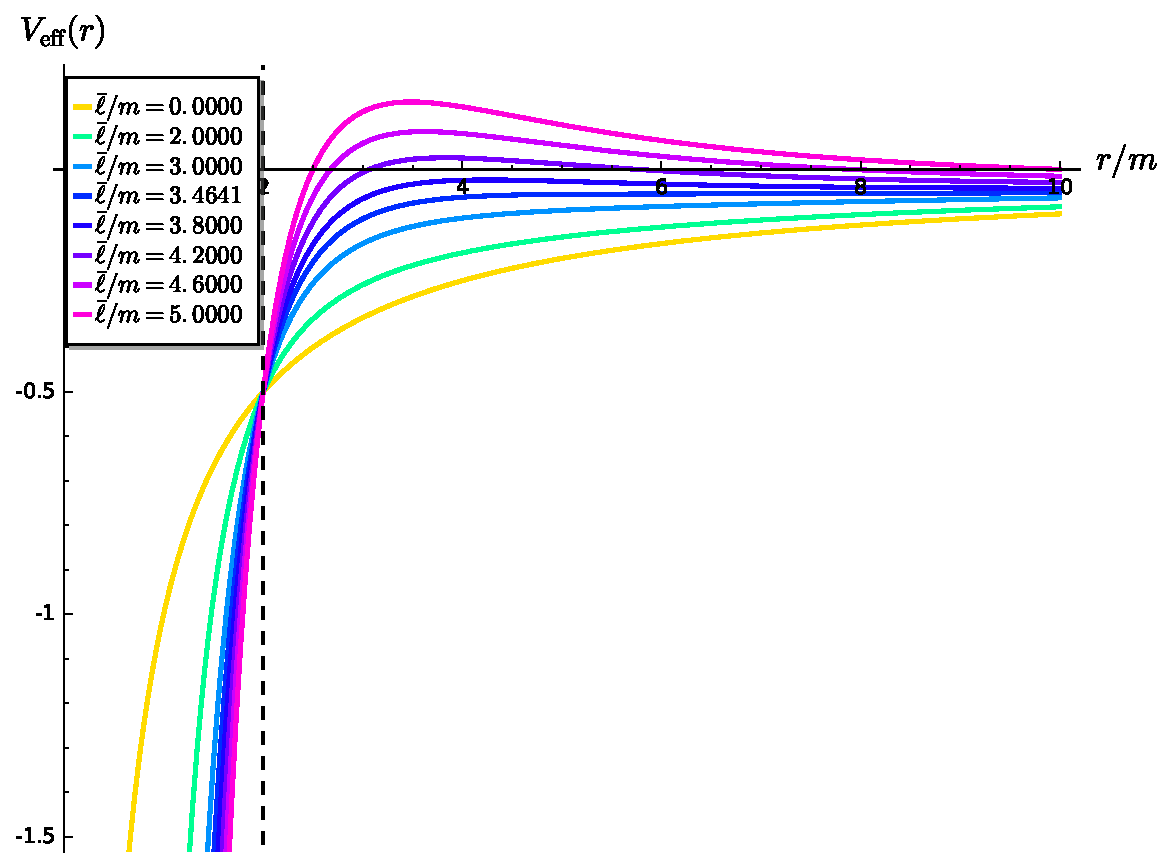
\includegraphics[width=0.8\textwidth]{ges_eff_pot.pdf}}
\caption[]{\label{f:ges:eff_pot} \footnotesize
Effective potential $V_{\rm eff}(r)$ governing the radial motion along a timelike geodesic in
Schwarzschild spacetime. The vertical dashed line marks $r=2m$, i.e. the
location of the event horizon.
The numerical value $\bar{\ell}/m=3.4641$ is that of the critical
specific angular momentum (\ref{e:ges:ell_crit}).}
\end{figure}

\begin{figure}
\centerline{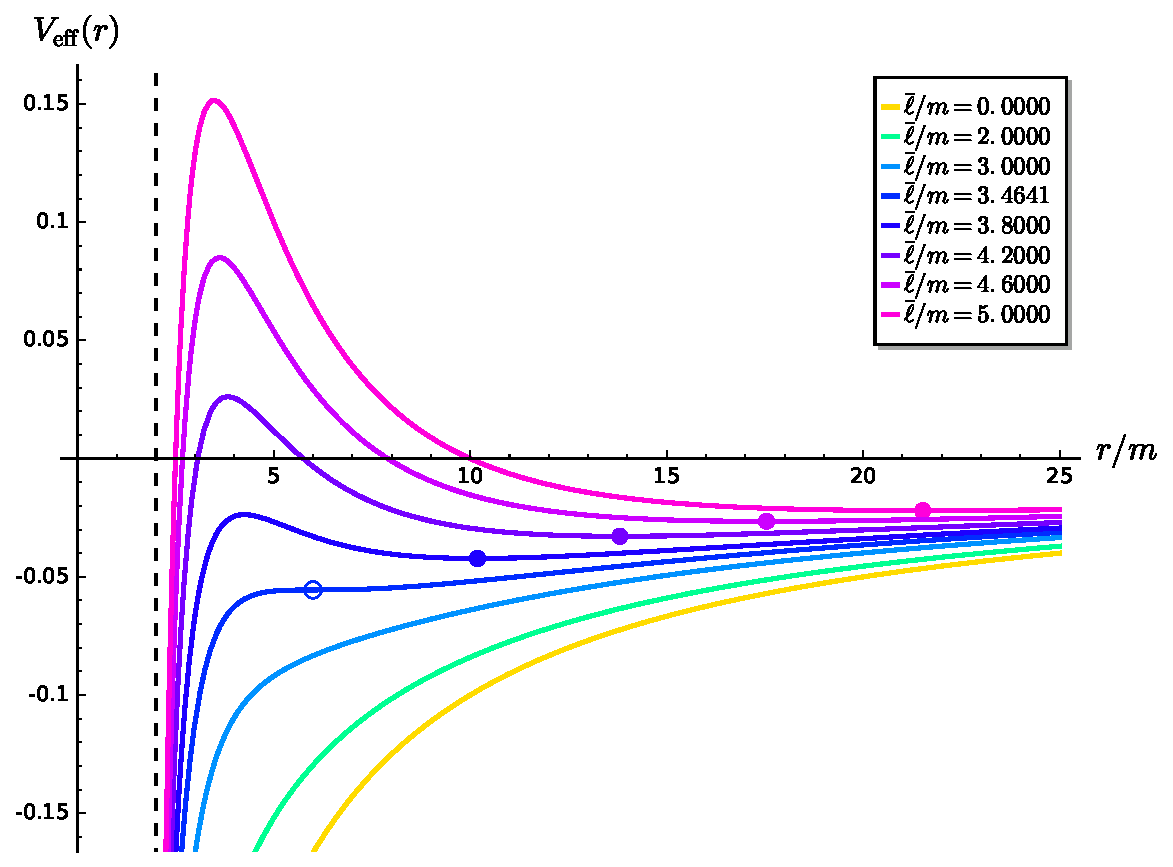
\includegraphics[width=0.8\textwidth]{ges_eff_pot_zoom.pdf}}
\caption[]{\label{f:ges:eff_pot_zoom} \footnotesize
Same as Fig.~\ref{f:ges:eff_pot}, but with a zoom in along the $y$-axis
and a zoom out along the $x$-axis. The dots mark the mimima of
$V_{\rm eff}$, locating stable circular orbits.}
\end{figure}

The profile  of $V_{\rm eff}(r)$ for selected values of $\bar{\ell}$ is
plotted in Figs.~\ref{f:ges:eff_pot} and \ref{f:ges:eff_pot_zoom} .
Its extrema are given by
$\D V_{\rm eff}/\D r=0$, which is equivalent to
\[
    m r^2 - \bar{\ell}^2 r + 3 \bar{\ell}^2 m = 0 .
\]
This quadratic equation admits real roots iff $|\bar{\ell}| \geq \bar{\ell}_{\rm crit}$,
with
\be \label{e:ges:ell_crit}
   \encadre{ \bar{\ell}_{\rm crit} = 2\sqrt{3} m }.
\ee
For $|\bar{\ell}| \geq \bar{\ell}_{\rm crit}$, the two roots are
\be
    r_{\rm max} = \frac{\bar{\ell}}{2m} \left( \bar{\ell} -
    \sqrt{\bar{\ell}^2 - \bar{\ell}_{\rm crit}^2} \right)
    \qquad\mbox{and}\qquad
    r_{\rm min} = \frac{\bar{\ell}}{2m} \left( \bar{\ell} +
    \sqrt{\bar{\ell}^2 - \bar{\ell}_{\rm crit}^2} \right) ,
\ee
corresponding respectively to a maximum of $V_{\rm eff}$ and a minimum
of $V_{\rm eff}$, hence the indices ``max'' and ``min''. Note that
$r_{\rm max} \leq r_{\rm min}$.
In the marginal case $|\bar{\ell}| = \bar{\ell}_{\rm crit}$, the two roots
coincide and correspond to an inflection point of $V_{\rm eff}$ (the circled
dot in Fig.~\ref{f:ges:eff_pot_zoom}).

For $|\bar{\ell}| < \bar{\ell}_{\rm crit}$, there is no extremum and
$V_{\rm eff}$ is a scritly increasing function of $r$.


To get a full solution in terms of the Schwarzschild-Droste coordinates,
once Eq.~(\ref{e:ges:1d_motion_timelike}) is solved for $r(\tau)$,
one has still to solve Eqs.~(\ref{e:ges:dot_t}) and (\ref{e:ges:dot_ph}),
which can be rewritten in terms of the proper time $\tau$ as
\be \label{e:ges:Dt_Dtau}
    \frac{\D t}{\D \tau} = \bar{\veps} \left(1 - \frac{2m}{r(\tau)} \right) ^{-1} ,
\ee
\be \label{e:ges:Dph_Dtau}
    \frac{\D\ph}{\D\tau} = \frac{\bar{\ell}}{r(\tau)^2}  .
\ee


\subsection{Radial free fall} \label{s:ges:radial_free_fall}

\subsubsection{Generic case}

The radial geodesics correspond to a vanishing conserved angular momentum:
$\ell = 0$. Indeed, setting $\ell=0$ in Eq.~(\ref{e:ges:dot_ph}) yields
$\ph = \mathrm{const}$, which defines a purely radial trajectory in the
plane $\th=\pi/2$.
The effective potential (\ref{e:ges:V_eff_timelike}) reduces then
to $V_{\rm eff}(r) = - m/r$, so that the equation of radial motion
(\ref{e:ges:1d_motion_timelike}) becomes
\be \label{e:ges:radial_motion}
    \frac{1}{2} \left( \frac{\D r}{\D \tau} \right) ^2
        - \frac{m}{r} = \frac{\bar{\veps}^2 - 1}{2} .
\ee
This equation is identical to that governing radial free fall in the gravitational field generated by a mass $m$ in Newtonian gravity.
The solution is well known and
depends on the sign of the ``mechanical energy'' in the right-hand
side, i.e. of the position of $\bar{\veps}$ with respect to $1$, or
equivalently of that of the conserved energy $\veps$ with respect
to the particle's mass $\mu$:
\begin{itemize}
\item if $\veps>\mu$, the solution
is given in parametrized form (parameter $\eta$) by
\be \label{e:ges:sol_E_pos}
    \left\{ \begin{array}{l}
    \displaystyle\tau = \frac{m}{(\bar{\veps}^2 - 1)^{3/2}} \left( \sinh\eta - \eta \right)
        + \tau_0 \\[2ex]
    \displaystyle r = \frac{m}{\bar{\veps}^2 - 1} \left( \cosh\eta - 1 \right),
    \end{array} \right.
\ee
\item if $\veps=\mu$, the solution is
\be \label{e:ges:sol_E_zero}
    r(\tau) =  \left( \frac{9 m}{2} (\tau -\tau_0)^2 \right) ^{1/3} ,
\ee
\item if $\veps<\mu$, the solution
is given in parametrized form (parameter $\eta$) by
\be \label{e:ges:sol_E_neg}
    \left\{ \begin{array}{l}
    \displaystyle\tau =  \frac{m}{|\bar{\veps}^2 - 1| ^{3/2}} \left( \eta + \sin\eta \right)
    + \tau_0  \\[2ex]
    \displaystyle r = \frac{m}{|\bar{\veps}^2 - 1|} \left( 1 + \cos\eta \right),
    \end{array} \right.
\ee
\end{itemize}
In the above formulas, $\tau_0$ is a constant; for $\veps\geq \mu$,
it sets the value of $\tau$ for which $r\rightarrow 0$, while
for $\veps<\mu$, it sets the value of $\tau$ at which $r$ takes its maximal value.

\subsubsection{Radial free fall from rest}

Let us focus on the radial free fall from rest, starting at some
position $r=r_0$ at $\tau=0$. Starting from rest
means $\D r/\D\tau = 0$ at $\tau=0$. The equation of radial motion
(\ref{e:ges:radial_motion}) leads then to $-m/r_0 = (\bar{\veps}^2 - 1)/2$,
or equivalently
\be \label{e:ges:beps2}
         \bar{\veps}^2 = 1 - \frac{2m}{r_0} .
\ee
The right-hand side of this equation must be non-negative. This implies
$r_0\geq 2m$. We recover the fact that one cannot be momentarily at rest
(in terms of $r$) if $r_0<2m$, for $r$ has to decrease along any future-directed
worldline in the black hole region $\M_{\rm II}$ (cf. Sec.~\ref{s:sch:time_orientation}).

Equation~(\ref{e:ges:beps2}) implies $\bar{\veps} < 1$, i.e. $\veps < \mu$. The solution
is thus given by Eq.~(\ref{e:ges:sol_E_neg}); expressing $|\bar{\veps}^2 - 1|$
in it via (\ref{e:ges:beps2}), we get
\be \label{e:ges:sol_radial_infall}
    \encadre{
    \left\{ \begin{array}{l}
    \displaystyle\tau = \sqrt{\frac{r_0^3}{8 m}}  \left( \eta + \sin\eta \right) \\[3ex]
    \displaystyle r = \frac{r_0}{2} \left( 1 + \cos\eta \right)
    \end{array} \right. }
    \qquad 0 \leq \eta \leq \pi ,
\ee
where the range of $\eta$ is such that $r=r_0$ for $\tau=0$ ($\eta=0$) and
$r$ decays to $0$ when $\eta\rightarrow \pi$. The function $r(\tau)$ resulting
from (\ref{e:ges:sol_radial_infall}) is depicted in
Fig.~\ref{f:ges:radial_infall_tau}.

\begin{figure}
\centerline{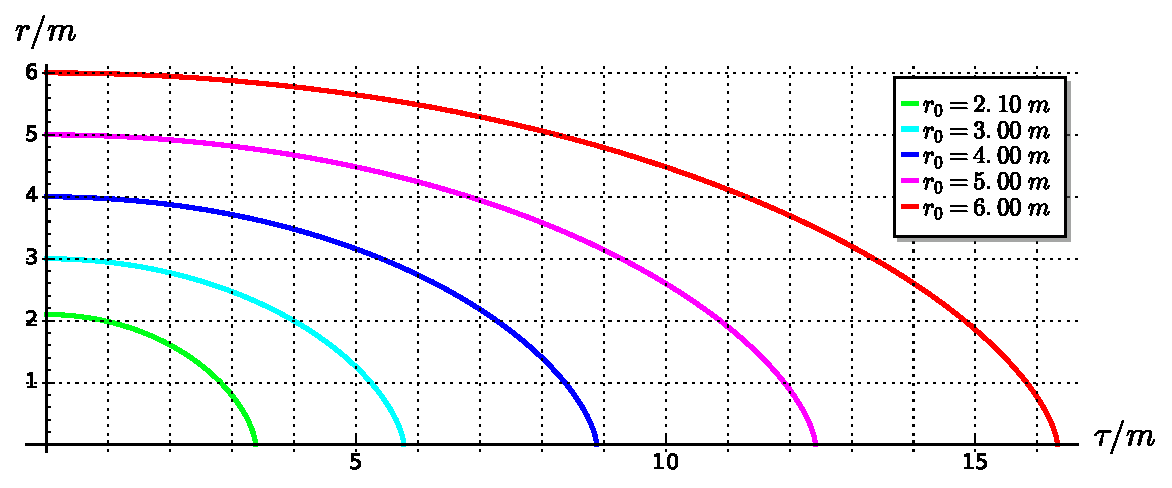
\includegraphics[width=0.8\textwidth]{ges_radial_infall_tau.pdf}}
\caption[]{\label{f:ges:radial_infall_tau} \footnotesize
Coordinate $r$ as a function of the proper time $\tau$
for the radial free fall from rest, for various initial values $r_0$ of $r$.}
\end{figure}

The solution for $t=t(\tau)$ is obtained by combining $\D t/\D\tau$ as expressed
by (\ref{e:ges:Dt_Dtau}) and $\D\tau/\D\eta$ deduced from (\ref{e:ges:sol_radial_infall}):
\[
    \frac{\D\tau}{\D\eta} = \sqrt{\frac{r_0^3}{8 m}}  \left( 1 + \cos\eta \right)
        = \sqrt{\frac{r_0}{2m}} \, r .
\]
We get
\[
    \frac{\D t}{\D\eta} =  \frac{\D t}{\D\tau} \frac{\D\tau}{\D\eta}
        = \bar{\veps} \sqrt{\frac{r_0}{2m}} \, r \left(1 - \frac{2m}{r} \right) ^{-1}
        = \sqrt{\frac{r_0}{2m} - 1} \; \frac{r^2}{r - 2m} ,
\]
where we have used (\ref{e:ges:beps2}) and $\bar{\veps} > 0$ to write
$\bar{\veps} = \sqrt{1-2m/r_0}$.
Substituting $r$ from Eq.~(\ref{e:ges:sol_radial_infall}), we get
\[
    \frac{\D t}{\D\eta} =   \frac{r_0}{2} \sqrt{\frac{r_0}{2m} - 1} \;
        \frac{(1+\cos\eta)^2}{1+\cos\eta - 4m/r_0} .
\]
This equation can be integrated to (cf. the \textsf{SageMath} computation in Sec.~\ref{s:sam:ges_radial_free_fall})
\be \label{e:ges:sol_t_radial_infall}
   \encadre{ t = 2m \left\{ \sqrt{\frac{r_0}{2m} - 1} \left[ \eta + \frac{r_0}{4m}
    (\eta + \sin\eta) \right]
    + \ln \left| \frac{\sqrt{\frac{r_0}{2m} - 1} + \tan\frac{\eta}{2}}{\sqrt{\frac{r_0}{2m} - 1} - \tan\frac{\eta}{2}} \right| \right\} } ,
\ee
where we have assumed $t=0$ at $\tau=0$ ($\eta=0$).

\begin{figure}
\centerline{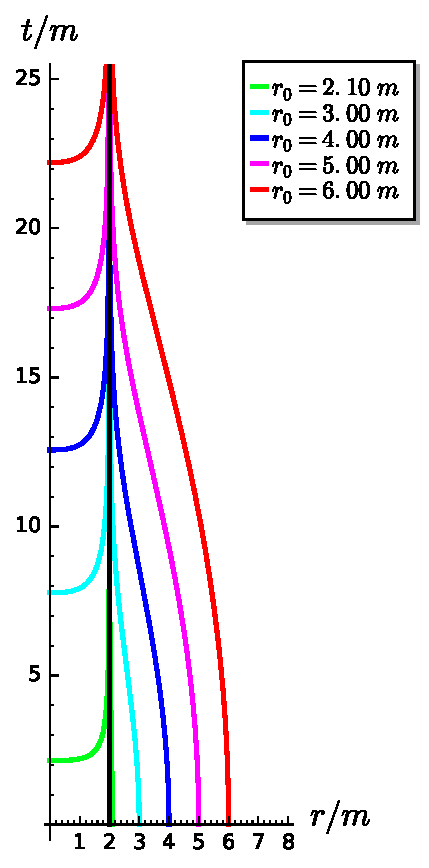
\includegraphics[height=0.5\textheight]{ges_radial_infall_t.pdf}\qquad\qquad
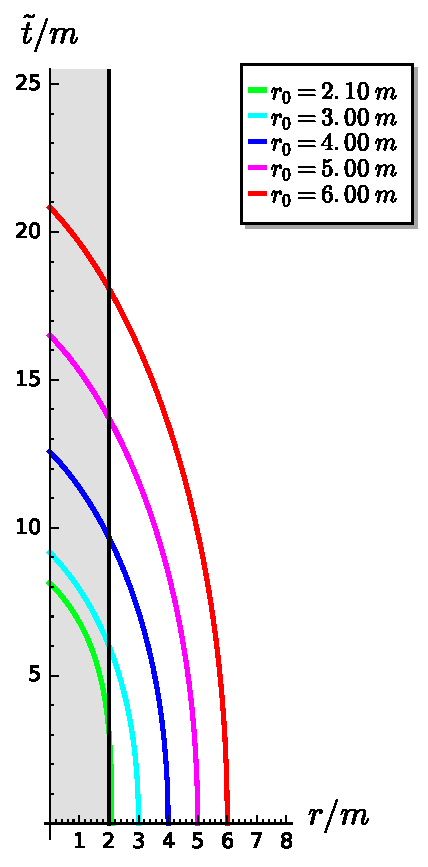
\includegraphics[height=0.5\textheight]{ges_radial_infall_IEF.pdf}}
\caption[]{\label{f:ges:radial_infall} \footnotesize
Radial free fall from rest, viewed in Schwarzschild-Droste coordinates $(t,r)$
(left) and in the ingoing Eddington-Finkelstein coordinates $(\ti,r)$ (right),
for various values $r_0$ of the coordinate $r$ at $\tau=0$. The grey area is the
black hole region $\M_{\rm II}$.}
\end{figure}


The solution of the radial free fall starting from rest at $r=r_0$ is
thus given in parametric form by Eqs.~(\ref{e:ges:sol_radial_infall}) and
(\ref{e:ges:sol_t_radial_infall}) and is represented in the left panel
of Fig.~\ref{f:ges:radial_infall}. It has been obtained in the Schwarzschild-Droste coordinates
$(t,r,\th,\ph)$, which are singular at the event horizon $\Hor$. So, one might wonder
if such a solution can describe the full infall, with the crossing of $\Hor$.
In particular, we notice that the differential equation for $t(\tau)$,
Eq.~(\ref{e:ges:Dt_Dtau}), is singular at $r(\tau)=2m$, i.e. on $\Hor$. The solution
$t(\eta)$, as given by Eq.~(\ref{e:ges:sol_t_radial_infall}), is singular at
$\eta=\eta_{\rm h}$, where
\be \label{e:ges:def_eta_star}
    \eta_{\rm h} := 2 \,\mathrm{atan}\, \sqrt{\frac{r_0}{2m} - 1}
\ee
is precisely the value of $\eta$ yielding $r=2m$ in Eq.~(\ref{e:ges:sol_radial_infall})
[to see it, rewrite the second part of Eq.~(\ref{e:ges:sol_radial_infall}) as
$r=r_0\cos^2(\eta/2) = r_0/(1+\tan^2(\eta/2))$].
This singularity of $t(\eta)$ appears also clearly on Fig.~\ref{f:ges:radial_infall} (left panel).
On the other hand, the equation
for $r$, Eq.~(\ref{e:ges:radial_motion}), does not exhibit any pathology
at $r=2m$, nor its solution (\ref{e:ges:sol_t_radial_infall}).
Actually, had we started from the ingoing Eddington-Finkelstein (IEF) coordinates
$(\ti,r,\th,\ph)$, instead of the Schwarzschild-Droste ones, we would have
found\footnote{{\emph Exercice:} do it!}
exactly the same solution for $r(\tau)$ (which is not surprising since
$r$, considered as a scalar field on $\M$, is perfectly regular at $\Hor$).
The solution for $\ti(\tau)$ can be deduced from that for $t(\tau)$ by
the coordinate transformation law (\ref{e:sch:ti_t_r}). Noticing that and
$r/(2m) = \cos^2(\eta/2)/\cos^2(\eta_{\rm h}/2)$, we get
\bea
    \frac{r}{2m} - 1 & = & \frac{\cos^2(\eta/2)}{\cos^2(\eta_{\rm h}/2)} - 1
        = \cos^2(\eta/2) \left( \frac{1}{\cos^2(\eta_{\rm h}/2)}
        - \frac{1}{\cos^2(\eta/2)} \right) \nonumber \\
       & = &\cos^2(\eta/2) \left(\tan^2(\eta_{\rm h}/2) - \tan^2(\eta/2) \right) .
\eea
Using this identity as well as (\ref{e:ges:def_eta_star}) to express
$\sqrt{r_0/(2m)-1}$ in Eq.~(\ref{e:ges:sol_t_radial_infall}), the transformation law (\ref{e:sch:ti_t_r}) yields
\bea
    \ti & = & 2m \left\{ \sqrt{\frac{r_0}{2m} - 1} \left[ \eta + \frac{r_0}{4m}
    (\eta + \sin\eta) \right]
    + \ln \left| \frac{\tan\frac{\eta_{\rm h}}{2} + \tan\frac{\eta}{2}}{\tan\frac{\eta_{\rm h}}{2}- \tan\frac{\eta}{2}} \cos^2\frac{\eta}{2} \left( \tan^2\frac{\eta_{\rm h}}{2}
        - \tan^2\frac{\eta}{2} \right) \right| \right\} \nonumber \\
    & = & 2m \left\{ \sqrt{\frac{r_0}{2m} - 1} \left[ \eta + \frac{r_0}{4m}
    (\eta + \sin\eta) \right]
    + \ln \left| \cos^2\frac{\eta}{2}
    \left( \tan\frac{\eta_{\rm h}}{2} + \tan\frac{\eta}{2} \right) ^2 \right| \right\} \nonumber \\
    & = & 2m \left\{ \sqrt{\frac{r_0}{2m} - 1} \left[ \eta + \frac{r_0}{4m}
    (\eta + \sin\eta) \right]
    +  2 \ln \left( \cos\frac{\eta}{2} \tan\frac{\eta_{\rm h}}{2} + \sin \frac{\eta}{2} \right) \right\} . \nonumber
\eea
From this expression, we have $\ti= 4 m \ln \tan(\eta_{\rm h}/2)$ for $\eta=0$.
Now, we can change the origin of the IEF coordinate $\ti$ to ensure $\ti=0$ for $\eta=0$,
i.e. $\tau=0$.
We get then
\be \label{e:ges:sol_radial_infall_ti}
    \encadre{ \ti = 2m \left\{ \sqrt{\frac{r_0}{2m} - 1} \left[ \eta + \frac{r_0}{4m}
    (\eta + \sin\eta) \right]
    +  2 \ln \left[ \cos\frac{\eta}{2}  + \left(\frac{r_0}{2m} - 1\right)^{-1/2} \sin \frac{\eta}{2} \right] \right\} } .
\ee
This expression is perfectly regular for all values of $\eta$ in $[0,\pi]$, reflecting
the fact that the ingoing Eddington-Finkelstein coordinates cover all $\M$
in a regular way. The radial free fall solution in terms of $(\ti, r)$
is represented in the right panel of Fig.~\ref{f:ges:radial_infall}. We note the
smooth crossing of the event horizon $\Hor$.

\begin{figure}
\centerline{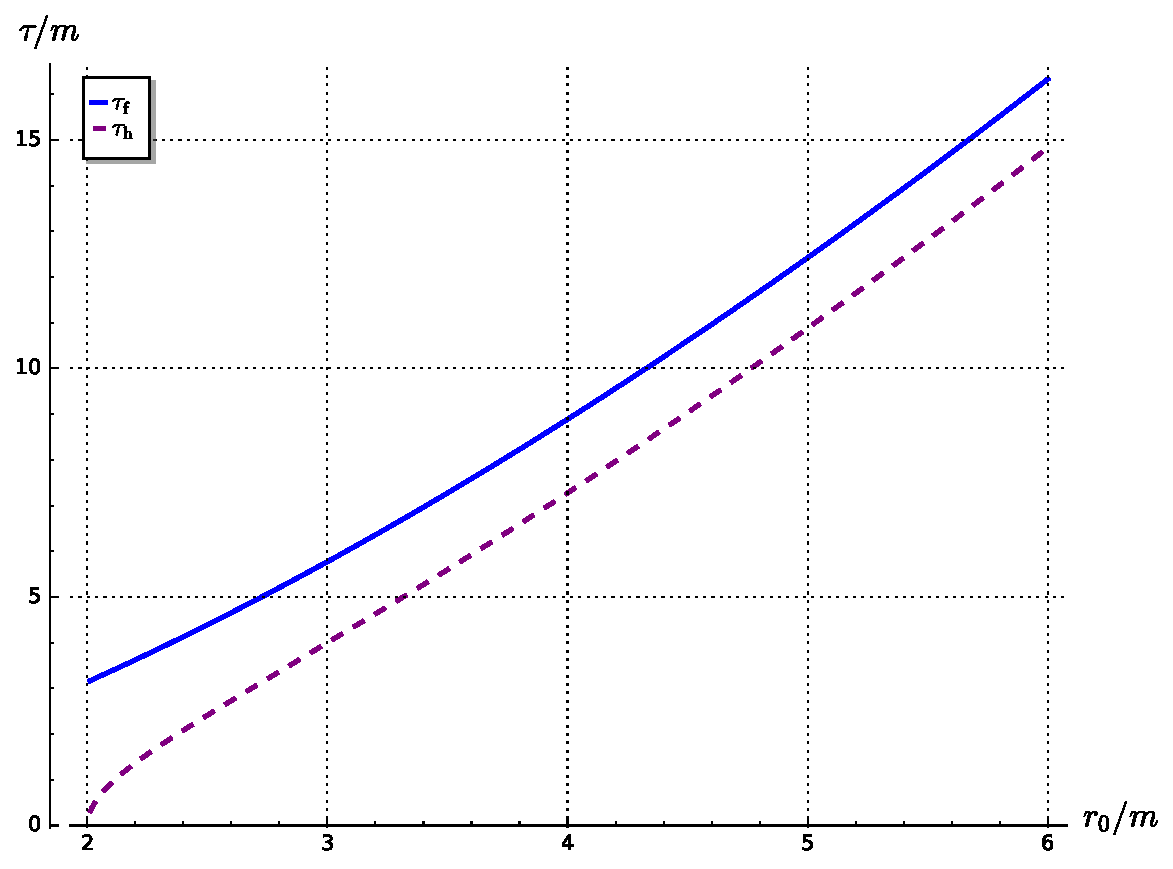
\includegraphics[height=0.4\textheight]{ges_infall_time.pdf}}
\caption[]{\label{f:ges:infall_time} \footnotesize
Elapsed proper time to reach the event horizon ($\tau_{\rm h}$, dashed curve)
and the central singularity ($\tau_{\rm f}$, solid curve), as a function
of the initial value of $r$ for a radial free fall from rest.}
\end{figure}

\begin{figure}
\centerline{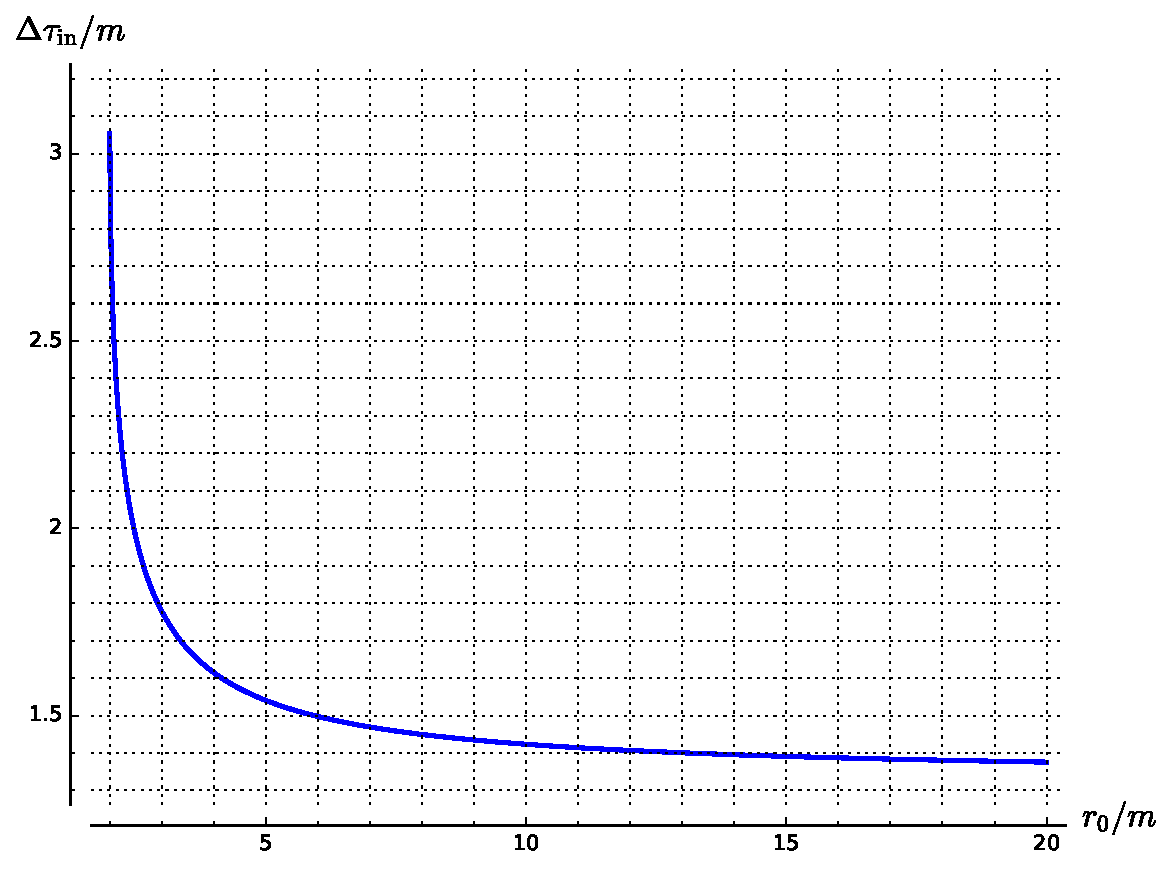
\includegraphics[height=0.4\textheight]{ges_time_inside.pdf}}
\caption[]{\label{f:ges:time_inside} \footnotesize
Proper time spent inside the black hole region as a function
of the initial value of $r$ for a radial free fall from rest.
Note that $r_0=2m$ does not correspond to an asymptote but to
a vertical tangent from the finite value $\Delta\tau_{\rm in} = \pi\, m$.
On the other side, there is the asymptotic value
$\Delta\tau_{\rm in} \rightarrow 4m/3$ for $r_0\rightarrow +\infty$.}
\end{figure}

In view of Eq.~(\ref{e:ges:sol_radial_infall}), we may say that the radial
infall starts at $\eta=0$, for which $\tau=0$ and $r=r_0$, and terminates
at $\eta=\pi$, for which $r=0$, which means that the particle hits the curvature
singularity. The final value of the particle's proper time is obtained by
setting $\eta=\pi$ in Eq.~(\ref{e:ges:sol_radial_infall}):
\be
    \encadre{\tau_{\rm f} = \frac{\pi}{2} \sqrt{\frac{r_0^3}{2 m}} } .
\ee
Similarly, the final value of $\ti$ is obtained by setting $\eta=\pi$ in (\ref{e:ges:sol_radial_infall_ti}):
\be
    \encadre{\ti_{\rm f} = 2 m \left[ \pi \sqrt{\frac{r_0}{2m} - 1 }
        \left( \frac{r_0}{4m} + 1 \right)
        -  \ln  \left( \frac{r_0}{2m} - 1 \right) \right] } .
\ee
As noticed above, the event horizon $\Hor$ is crossed at $\eta=\eta_{\rm h}$;
via (\ref{e:ges:sol_radial_infall}) and (\ref{e:ges:def_eta_star}), this corresponds to the following value
of the proper time:
\be
    \encadre{\tau_{\rm h} = \sqrt{\frac{r_0^3}{2m}}
        \left[ \mathrm{atan}\, \sqrt{\frac{r_0}{2m} - 1} +
        \sqrt{\frac{2m}{r_0} \left( 1 - \frac{2m}{r_0} \right) } \right] } ,
\ee
while (\ref{e:ges:sol_radial_infall_ti}) leads to the following value
of the IEF coordinate $\ti$:
\be
    \encadre{\ti_{\rm h} = 2m \left[ 2\left(1+\frac{r_0}{4m}\right)
        \sqrt{\frac{r_0}{2m} - 1} \, \mathrm{atan}\, \sqrt{\frac{r_0}{2m} - 1}
        + \frac{r_0}{2m} - 1 - \ln\frac{r_0}{2m} \right] } .
\ee
The variation of $\tau_{\rm h}$ and $\tau_{\rm f}$ with $r_0$ are depicted in
Fig.~\ref{f:ges:infall_time} and numerical values for $r_0=6m$ and
standard astrophysical black holes are provided in
Table~\ref{t:ges:time_free_fall}.

\begin{table}
\centerline{
\begin{tabular}{c|c|c|c|c}
\hline
$m$ & $r_{\rm S} = 2m$ & $\tau_{\rm h}$ & $\tau_{\rm f}$ & $\Delta\tau_{\rm in}$ \\[0.5ex]
\hline\hline
$15\, M_\odot$ (Cyg X-1) & $44.3 {\rm\; km}$ & $1.10 {\rm\; ms}$ & $1.21 {\rm\; ms}$ & $0.11 {\rm\; ms}$ \\[0.5ex]
\hline
$4\; 10^6 \, M_\odot$ (Sgr A*) & $11.8\; 10^6 {\rm\; km}$ & $4 {\rm\; min\; } 52 {\rm\; s}$ & $6 {\rm\; min\; } 22 {\rm\; s}$ & $30 {\rm\; s}$ \\[0.5ex]
\hline
$6\; 10^9 \, M_\odot$ (M 87) & $118 {\rm\; UA}$ & $5.07 {\rm\; days}$ & $5.58 {\rm\; days}$ & $12 {\rm\; h\;} 17 {\rm\; min}$ \\[0.5ex]
\hline
\end{tabular}
}
\caption[]{\label{t:ges:time_free_fall} \footnotesize
Proper time to reach the event horizon ($\tau_{\rm h}$), to reach
the central curvature singularity ($\tau_{\rm f}$) and elapsed proper
time inside the black hole region ($\Delta\tau_{\rm in}$), when freely falling
from rest at $r_0 = 6m$. The numerical values are given for various
black hole masses $m$, corresponding to astrophysical objects:
a stellar black hole (Cyg X-1), the black hole at the center of our galaxy
(Sgr A*) and the massive black hole in the nucleus of the galaxy M~87.}
\end{table}

The proper time spent inside the black hole is
\be
    \encadre{\Delta\tau_{\rm in}  = \tau_{\rm f} - \tau_{\rm h}
    = \sqrt{\frac{r_0^3}{2m}}
        \left[ \frac{\pi}{2} - \mathrm{atan}\, \sqrt{\frac{r_0}{2m} - 1} -
        \sqrt{\frac{2m}{r_0} \left( 1 - \frac{2m}{r_0} \right) } \right] } .
\ee
It varies between $\pi m$ ($r_0 \rightarrow 2m$) and $4m/3$ ($r_0 \rightarrow +\infty$)
(cf. Fig.~\ref{f:ges:time_inside} and Sec.~\ref{s:sam:ges_radial_free_fall}
for the computation of $\lim_{r_0\rightarrow +\infty} \Delta\tau_{\rm in}$).
Numerical values for standard astrophysical black holes are provided in
Table~\ref{t:ges:time_free_fall}.

%%%%%%%%%%%%%%%%%

\subsection{Circular orbits}\index{circular!orbit}\index{orbit!circular --}

Circular orbits are defined as timelike geodesics with $r = \mathrm{const}$.
We have then $\D r/\D\tau = 0$ and $\D^2 r/\D\tau^2 = 0$.
Equation~(\ref{e:ges:1d_motion_timelike}) implies then for such orbits
\begin{subequations}
\begin{align}
& V_{\rm eff}(r) = \frac{\bar{\veps}^2 - 1}{2} \label{e:ges:Veff_circ} \\
& \frac{\D V_{\rm eff}}{\D r} = 0 . \label{e:ges:dVeffdr_zero}
\end{align}
\end{subequations}
Given the expression (\ref{e:ges:V_eff_timelike}) of $V_{\rm eff}$,
Eq.~(\ref{e:ges:dVeffdr_zero}) is equivalent to
\be \label{e:ges:eq_r_ell_circ}
    m r^2 - \bar{\ell}^2 r + 3 \bar{\ell}^2 m = 0 .
\ee
As already noticed in Sec.~\ref{s:ges:eff_pot_timelike}, this
quadratic equation in $r$ admits real roots iff $|\bar{\ell}| \geq \bar{\ell}_{\rm crit}$,
with $\bar{\ell}_{\rm crit} = 2\sqrt{3}\, m$ [Eq.~(\ref{e:ges:ell_crit})].
The two roots are then
\be \label{e:ges:r_circ_ell}
    \encadre{ r_{\rm circ}^\pm(\bar{\ell}) = \frac{\bar{\ell}^2}{2m} \left(
     1 \pm \sqrt{1 - \left( \frac{\bar{\ell}_{\rm crit}}{\bar{\ell}} \right) ^2 } \right) }.
\ee
$r_{\rm circ}^+(\bar{\ell})$ corresponds to a minimum of the effective potential
$V_{\rm eff}$ and thus
to a stable orbit (see the dots in Fig.~\ref{f:ges:eff_pot_zoom}),
while $r_{\rm circ}^-(\bar{\ell})$ corresponds to a
maximum of $V_{\rm eff}$ and thus to an unstable orbit.
When $\bar{\ell}$ varies from $\bar{\ell}_{\rm crit}$ to $+\infty$,
$r_{\rm circ}^+(\bar{\ell})$ increases from $6 m$ to $+\infty$, while
$r_{\rm circ}^-(\bar{\ell})$ decreases from $6 m$ to $3 m$ (cf. Fig.~\ref{f:ges:ell_circ_orbit}). We conclude that
\begin{greybox}
Circular orbits in Schwarzschild spacetime exist for all values of $r>3m$.
Those with $r<6m$ are unstable and those with $r>6m$ are stable. The marginal
case $r=6m$ is called the \defin{innermost stable circular orbit}\index{stable!circular orbit}, often abriged as \defin{ISCO}\index{ISCO}.
\end{greybox}

\begin{figure}
\centerline{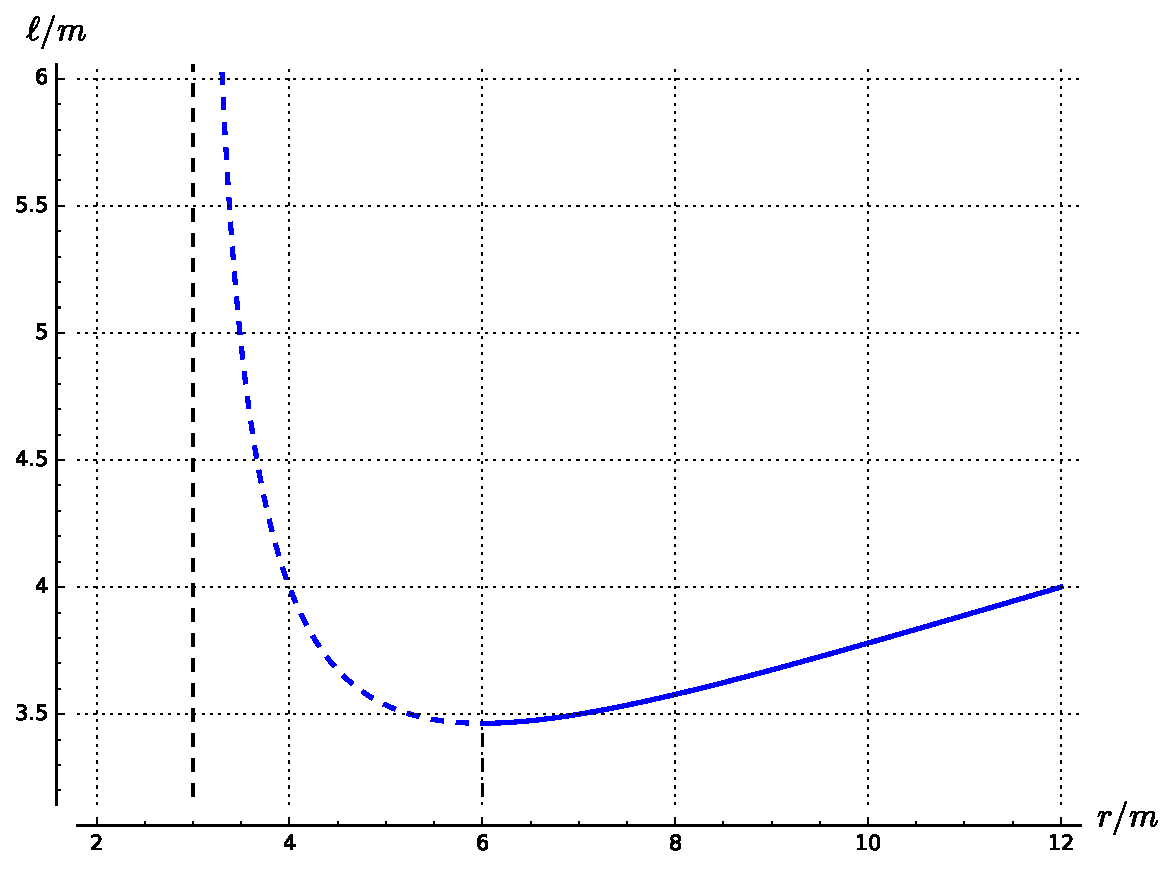
\includegraphics[height=0.4\textheight]{ges_ell_circ_orbit.pdf}}
\caption[]{\label{f:ges:ell_circ_orbit} \footnotesize
Specific conserved angular momentum $\bar{\ell} = \ell/\mu$
on circular orbits as a function of the
orbit circumferential radius $r$. The dashed part of the curve
corresponds to unstable orbits ($r=r_{\rm circ}^-(\bar{\ell})$, as given by Eq.~(\ref{e:ges:r_circ_ell})), while
the solid part corresponds to stable orbits ($r=r_{\rm circ}^+(\bar{\ell})$).
The minimal value of $\bar{\ell}$ is $\bar{\ell}_{\rm crit} = 2\sqrt{3}\, m \simeq 3.46\, m$.}
\end{figure}

From Eq.~(\ref{e:ges:eq_r_ell_circ}), we can easily express $\bar{\ell}$
as a function of $r$ on a circular orbit:
\be \label{e:ges:ell_r_circ}
    \encadre{ |\bar{\ell}| = r \sqrt{\frac{m}{r - 3m}} } .
\ee
This function is represented in Fig.~\ref{f:ges:ell_circ_orbit} (for $\bar{\ell} > 0$).

If we substitute (\ref{e:ges:ell_r_circ}) for $\bar{\ell}$ in
the expression (\ref{e:ges:V_eff_timelike}) of $V_{\rm eff}$
and use Eq.~(\ref{e:ges:Veff_circ}), we obtain the value of the
specific conserved energy along a circular orbit, in terms of $r$:
\be \label{e:ges:eps_r_circ}
    \encadre{ \bar{\veps} = \frac{r - 2m}{\sqrt{r(r-3m)}} } .
\ee
This function is represented in Fig.~\ref{f:ges:ener_circ_orbit}.
The minimal value of $\bar{\veps}$ is achieved for $r=6m$, i.e. at the ISCO:
\be
    \encadre{ \mathrm{min}\,  \bar{\veps} = \frac{2\sqrt{2}}{3} \simeq 0.9428} .
\ee
We notice that
\be
    r > 4 m \iff \bar{\veps} < 1 \iff \veps < \mu .
\ee
This corresponds to \defin{bound orbits}\index{bound!orbit}\index{orbit!bound --},
is to geodesics that, if slightly pertubed, cannot reach the asymptotically
flat region $r\gg 2m$, since $\veps \geq \mu$ there. Indeed, when
$r\rightarrow +\infty$, the Killing vector $\w{\xi}$ can be interpreted
as the 4-velocity of some asymptotically inertial observer (at rest with
respect to the black hole) and $\veps$ is the particle energy measured by
that observer; the famous Einstein relation (\ref{e:fra:E_Gam_m}) is then
$\veps = \Gamma \mu$, where $\Gamma$ is the Lorentz factor
of the particle with respect to the observer.
Since $\Gamma \geq 1$ [Eq.~(\ref{e:fra:Gam_V2})], we have obviously\footnote{Similarly,
the radial-motion solutions (\ref{e:ges:sol_E_pos})-(\ref{e:ges:sol_E_zero}), which
allow for $r\rightarrow +\infty$, have $\veps\geq\mu$, while the solution (\ref{e:ges:sol_E_neg}),
which is relevant for a free fall from rest, has $\veps < \mu$.} $\veps \geq \mu$.
For this reason, the circular orbit at $r=4m$ is called the
\defin{marginally bound orbit}\index{marginally bound!orbit}\index{orbit!marginally bound --}. Note that the marginally bound orbit is unstable, since it has $r<6m$.

\begin{figure}
\centerline{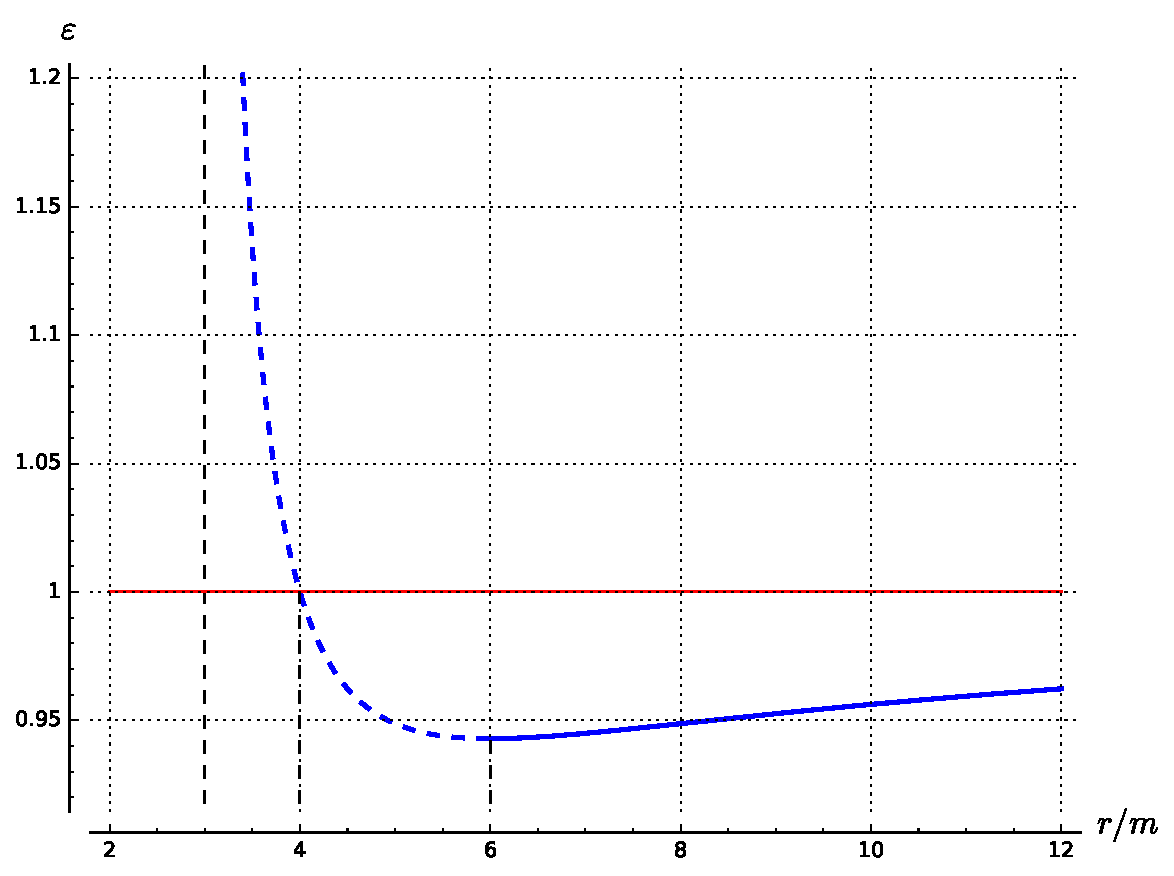
\includegraphics[height=0.4\textheight]{ges_ener_circ_orbit.pdf}}
\caption[]{\label{f:ges:ener_circ_orbit} \footnotesize
Specific conserved energy $\bar{\veps} = \veps/\mu$
on circular orbits as a function of the
orbit circumferential radius $r$.
The dashed part of the curve
corresponds to unstable orbits,
while the solid part corresponds to stable ones.
The horizontal red line marks the limit of bound orbits ($\veps=\mu$).}
\end{figure}

The \defin{angular velocity}\index{angular!velocity} of a circular orbit $\Li$ is defined by
\be \label{e:ges:def_Omega}
    \Omega := \left. \frac{\D\ph}{\D t} \right| _\Li = \frac{u^\ph}{u^t} ,
\ee
where $u^\ph = \D\ph/\D\tau$ and $u^t = \D t/\D\tau$ are the only
nonzero components w.r.t. Schwarzschild-Droste coordinates
of the 4-velocity $\w{u}$ of the particle $\mathscr{P}$ whose worldline is
$\Li$. It follows from (\ref{e:ges:def_Omega}) that
$\Omega$ enters into the linear combination of the two Killing
vectors $\w{\xi}$ and $\w{\eta}$ expressing the 4-velocity on a circular
orbit according to
\be
    \w{u} = u^t\left( \w{\xi} + \Omega \w{\eta} \right) .
\ee
The quantity $\Omega$ has a nice physical meaning: it is nothing but
the angular velocity of $\mathscr{P}$ monitored by a distant static
observer $\Obs$.
\begin{proof}
Suppose that $\Obs$ is located at fixed coordinates
$(r,\th,\ph)=(r_\Obs,\pi/2,0)$ with $r_\Obs\gg m$ and that
$\mathscr{P}$ emits a photon at the event
$(t_1, r, \pi/2, 0)$ along a \emph{radial} null geodesic. This photon is received
by $\Obs$ at $t=t'_1$. After one orbit, at the event $(t_2, r, \pi/2, 0)$,
$\mathscr{P}$ emits a second photon in the radial direction, which is received
at $t=t'_2$ by $\Obs$. According to the definition (\ref{e:ges:def_Omega})
of $\Omega$, we have
\[
    2\pi = \Omega(t_2 - t_1) .
\]
On the other hand, since $r_\Obs\gg m$, the proper time of $\Obs$ is $t$, so that the
angular velocity measured by $\Obs$ is
\[
    \Omega_\Obs = \frac{2\pi}{t'_2 - t'_1} .
\]
Now, since $t$ is the coordinate associated to
the spacetime invariance by time translation (stationarity), we have
necessarily $t'_2 - t'_1 = t_2 - t_1$. Accordingly, the above two equations
combine to $\Omega_\Obs = \Omega$.
\end{proof}

By combining Eqs.~(\ref{e:ges:Dt_Dtau}) and (\ref{e:ges:Dph_Dtau}), we get
\[
    \Omega = \frac{1}{r^2} \left( 1 -\frac{2m}{r} \right) \frac{\bar{\ell}}{\bar{\veps}} .
\]
Substituting expression (\ref{e:ges:ell_r_circ}) for $\bar{\ell}$ and
expression (\ref{e:ges:eps_r_circ}) for $\bar{\veps}$, we obtain
\be \label{e:ges:Omega_m_r}
    \encadre{ \Omega = \sqrt{\frac{m}{r^3}} } .
\ee
\begin{remark}
This formula is identical to that of Newtonian gravity (Kepler's third law for circular
orbits), but it is a mere coincidence.
\end{remark}

\begin{remark}
$\Omega$ is not the orbital angular frequency experienced by the particle/observer
$\mathscr{P}$ on the circular orbit $\Li$, because the proper time of $\mathscr{P}$ is
$\tau$ and not $t$. The actual orbital frequency measured by $\mathscr{P}$
is
\[
    \Omega_{\mathscr{P}} = \frac{\D t}{\D \tau} \Omega = u^t \Omega ,
\]
with $u^t = \D t/\D\tau$ obtained from (\ref{e:ges:Dph_Dtau}) and
(\ref{e:ges:eps_r_circ}): $u^t = \sqrt{r/(r-3m)}$. Hence
\be
    \Omega_{\mathscr{P}} = \sqrt{\frac{r}{r-3m}}\, \Omega  =
       \frac{1}{r}\sqrt{\frac{m}{r-3m}} .
\ee
We notice that $\Omega_{\mathscr{P}} > \Omega$.
\end{remark}

At the ISCO, $r=6m$ and formula (\ref{e:ges:Omega_m_r}) yields
\be
    \encadre{ \Omega_{\rm ISCO} = \frac{1}{6\sqrt{6}\, m} } .
\ee


\section{Null geodesics}


\begin{hist}
Synge \cite{Synge66}, Bardeen \cite{Barde73}
\end{hist}
